\documentclass[urlrm]{usmthesis}
%%%%%%%%%%%%%%%%%%%%%%%%%%%%%%%%%%%%%%%%%%%%%%%%%%%%%%%
% This is usmthesis.tex, Nov 27 2007.
% Created by Lim Lian Tze,
% Computer Aided Translation Unit,
% School of Computer Sciences, 
% Universiti Sains Malaysia, Penang, Malaysia.
%
% This is the "main" file for the thesis, 
% formatted according to the Guide to the 
% Preparation, Submission and Examination of
% Theses, published by IPS USM.
%%%%%%%%%%%%%%%%%%%%%%%%%%%%%%%%%%%%%%%%%%%%%%%%%%%%%%%

%% Example of loading other packages that you may require.
%% I'm loading the marvosym package so that I can produce a
%% smiley face with the command \Smiley.
%%\usepackage{marvosym}

%% Enter particulars about your thesis HERE
% Your Name
\author{Chong Chee Kang}
% English title of your thesis
\title{Electric Drive Optimisation}
% Malay title of your thesis
%%\titlems{Penulisan Tesis dengan LaTeX}
% Year submitted
\submityear{2012}
% Month submitted
\submitmonth{June}
%% Choose only 1 degree type! :-)
%\degreetype{Doctor of Philosphy}
\degreetype{Bachelor of Engineering (Mechanical Engineering)}
% Supervisor name
\supervisor{Prof. Horizon Walker Gitano-Briggs}
% Matrix Number
\matrixnum{102449}


%%%%%%%%%%%%%%%%%%%%%%%%%%%%%%%%%%%%%%%%%%%%%%%%%%%%%%%
%  You can comment out the following line if you don't have a
% "List of Own Publications"
%%%%%%%%%%%%%%%%%%%%%%%%%%%%%%%%%%%%%%%%%%%%%%%%%%%%%%%
%\newcites{own}{List of Publications}

%%%%%%%%%%%%%%%%%%%%%%%%%%%%%%%%%%%%%%%%%%%%%%%%%%%%%%%
% Options for generating hyperlinks when using pdfLaTeX
%%%%%%%%%%%%%%%%%%%%%%%%%%%%%%%%%%%%%%%%%%%%%%%%%%%%%%%
%%\ifpdf
%%  \makeatletter
%%  \usepackage[pdftex,plainpages=false,hypertexnames=false,bookmarksnumbered,pdfpagelabels,%
%%    pdfauthor={\@author},pdftitle={\@title}]{hyperref}
%%  \makeatother
%%\else
%%  \usepackage[dvips,plainpages=false,bookmarksnumbered,breaklinks=true]{hyperref}
%%\fi

%%pdf bookmark
\usepackage[pdftex,bookmarks=true]{hyperref}
\usepackage{textcomp}
\usepackage[Omega]{gensymb}

%%%%%%%%%%%%%%%%%%%%%%%%%%%%%%%%%%%%%%%%%%%%%%%%%%%%%%%
% As we have loaded the natbib package, you can customise
% the citation style to some extent.  The following line
% specifies some standard punctuations:
%
% \bibpunct{#1}{#2}{#3}{#4}{#5}{#6}
% #1: open punctuation (a round bracket here)
% #2: close punctuation (a round bracket here)
% #3: punctuation separating multiple authors (a semi-colon here)
% #4: n - citation using numerical system
%     s - numeric superscript system
%     any other letter - author-year system
% #5: punctuation separating author name(s) from year
% #6: punctuation separating years for multiple citations
%     with same author(s)
%
% The default citation that I used here is therefore of the form
% (Wilks and Stevenson, 1999; Somers, 2000)
%
% You may change any of the 6 parameters if you prefer a
% different citation style.  Also see the natbib documentation.
%%%%%%%%%%%%%%%%%%%%%%%%%%%%%%%%%%%%%%%%%%%%%%%%%%%%%%%
\bibpunct{(}{)}{;}{a}{,}{,}
\begin{document}

%%%%%%%%%%%%%%%%%%%%%%%%%%%%%%%%%%%%%%%%%%%%%%%%%%%%%%%
% You can choose from several bibliography styles. I'm using
% the author-year system with agsm for the bibliography
% entries here, but feel free to experiment with other styles.
%
% If you prefer the number system though, use bibliography
% style "plainnat" for [1][2][3] or "alpha" for [Jon94] (the label
% will be auto-generated).
%%%%%%%%%%%%%%%%%%%%%%%%%%%%%%%%%%%%%%%%%%%%%%%%%%%%%%%
%\bibliographystyle{dcu}
%\bibliographystyleown{dcu}
%\bibliographystyle{plainnat}
%\bibliographystyleown{plainnat}
\bibliographystyle{apalike}


\lstset{fontadjust=true}

\frontmatter

\addtocontents{lof}{\protect\raggedright\protect\sloppy}
\addtocontents{lof}{\protect\hfill{\protect\bfseries Page}\\}
\addtocontents{lot}{\protect\raggedright\protect\sloppy}
\addtocontents{lot}{\protect\hfill{\protect\bfseries Page}\\}
\addtocontents{equ}{\protect\raggedright\protect\sloppy}
\addtocontents{equ}{\protect\hfill{\protect\bfseries Page}\\}

%%%%%%%%%%%%%%%%%%%%%%%%%%%%%%%%%%%%%%%%%%%%%%%%%%%%%%%
% Inserts the cover page (the hard cover with gold-lettering)
% and the title page 
%%%%%%%%%%%%%%%%%%%%%%%%%%%%%%%%%%%%%%%%%%%%%%%%%%%%%%%
\makecover


%%%%%%%%%%%%%%%%%%%%%%%%%%%%%%%%%%%%%%%%%%%%%%%%%%%%%%%
% Inserts a "Front Matter" bookmark if using pdfLaTeX
%%%%%%%%%%%%%%%%%%%%%%%%%%%%%%%%%%%%%%%%%%%%%%%%%%%%%%%
%%\ifpdf
%%    \pdfbookmark[-1]{Front Matter}{front}
%%\else\fi

%%%%%%%%%%%%%%%%%%%%%%%%%%%%%%%%%%%%%%%%%%%%%%%%%%%%%%%
% Include the declaration
%%%%%%%%%%%%%%%%%%%%%%%%%%%%%%%%%%%%%%%%%%%%%%%%%%%%%%%
\chapter{Declaration}

This work has not previously been accepted in substance for any degree and is not being concurrently submitted in candidature for any degree.

\begin{flushleft}
Signed .............................................................. (Chong Chee Kang) \\ Date ..................................................
\end{flushleft}

\vspace{15mm}
\centerline{STATEMENT 1}
This thesis is the result of my own investigations, except where otherwise stated. Other sources are acknowledged by giving explicit references. References are appended.

\begin{flushleft}
Signed .............................................................. (Chong Chee Kang) \\ Date ..................................................
\end{flushleft}

\vspace{15mm}
\centerline{STATEMENT 2}
I hereby give consent for my thesis, if accepted, to be available for photocopying and for interlibrary loan, and for the title and summary to be made available outside organizations.

\begin{flushleft}
Signed .............................................................. (Chong Chee Kang) \\ Date ..................................................
\end{flushleft}


%%%%%%%%%%%%%%%%%%%%%%%%%%%%%%%%%%%%%%%%%%%%%%%%%%%%%%%
% MAKE SURE YOU HAVE A acknowledgements.tex FILE
%%%%%%%%%%%%%%%%%%%%%%%%%%%%%%%%%%%%%%%%%%%%%%%%%%%%%%%
\chapter{Acknowledgements}




\begin{singlespace}
\tableofcontents \clearpage
\listoftables \clearpage
\listoffigures \clearpage
\listofequations \clearpage
\end{singlespace}

%%%%%%%%%%%%%%%%%%%%%%%%%%%%%%%%%%%%%%%%%%%%%%%%%%%%%%%
% You can comment out the following line if you don't
% have a "List of Acronyms"
%%%%%%%%%%%%%%%%%%%%%%%%%%%%%%%%%%%%%%%%%%%%%%%%%%%%%%%
\chapter{List of Abbreviations}

\begin{acronym}[PMBLDC] %% replace 'MMMM' with the longest acronym in your list
\acro{AC}{Alternating Current}
\acro{BLDC}{Brushless DC}
\acro{DC}{Direct Current}
\acro{I/O}{Input Output}
\acro{PMBLDC}{Permanent Magnet Brushless DC}
\acro{PWM}{Pulse Width Modulation}
\acro{SOC}{State of Charge}
\end{acronym}


\chapter{List of Symbols}

\begin{acronym}[lim ]
\acro{lim}[$\lim{}$]{limit}
\end{acronym}



% Paragraph spacing
\setlength\parskip{18pt}
% Text-float spacing
\setlength\intextsep{24pt}

%%%%%%%%%%%%%%%%%%%%%%%%%%%%%%%%%%%%%%%%%%%%%%%%%%%%%%%
% Your Malay and English abstracts, each in one file.
%%%%%%%%%%%%%%%%%%%%%%%%%%%%%%%%%%%%%%%%%%%%%%%%%%%%%%%
\begin{MsAbstract}

Dalam Perlumbaan "Shell Eco-Marathon" kategori "Urban Concept", sebuah kereta yang serupa dengan kereta atas jalan dibina. Tertakluk kepada kategori yang disertai, yang dalam konteks ini kategori kereta elektrik "plug-in", motor electrik digunakan sebagai enjin kereta elektrik. Enjin kereta elektrik didirikan daripada pengawal dan sebuah "hub motor" yang disambung terus ke roda kereta, kedua-dua komponent tersebut adalah proprietari dan membukakan komponent tersebut dilarang sebab isu penajaan. Oleh itu, isyarat keluaran daripada pengawal iaitu voltan dan isyarat kelajuan telah dikenalpastikan untuk menubuhkan sebuah sistem pengukuran yang boleh digunakan untuk mengukur, mencatat dan memaparkan parameter tersebut. Sistem pengukuran tersebut ditubuhkan dengan menggunakan mikro-pengawal yang berjenama "Arduino", penghubung pemaparan ITDB02 dengan kad SD dan LCD skrin ITDB02-3.2WC untuk pemaparan. Selain daripada menggunakan sistem pengukuran untuk mengumpulkan data, perisian simulasi dinamik kenderaan yang berupaya mengsimulasikan rintangan rodaan, daya pengheretan, naik/turun cerun dan memandu serta mempercepatkan kenderaan dalam Sepang North Track dibina. Selepas itu, empat strategi untuk memandukan kereta tersebut dalam litar telah dibina bertujukan perjalanan paling jauh dengan tenaga yang paling kurang.  

\end{MsAbstract}

\begin{EnAbstract}
\end{EnAbstract}


\addtocontents{toc}{\protect\setlength{\protect\cftbeforechapskip}{2.5pc}}
\addtocontents{toc}{\protect\cftpagenumbersoff{chap}}
 
\mainmatter
%%\ifpdf
%%  \pdfbookmark[-1]{Main Chapters}{main}
%%\else\fi

%%%%%%%%%%%%%%%%%%%%%%%%%%%%%%%%%%%%%%%%%%%%%%%%%%%%%%%
% The actual chapters of your thesis as listed in 
% mainchaps.tex. Make sure you have the relevant
% chapter files. 
% E.g. if you mainchaps.tex contains the lines
%
%  \include{hypothesis.tex}
%  \include{proof.tex}
%
% Then you MUST have the files hypothesis.tex, proof.tex
% (containing the relevant chapters) in the same directory
% as mainchaps.tex.
%%%%%%%%%%%%%%%%%%%%%%%%%%%%%%%%%%%%%%%%%%%%%%%%%%%%%%%
\chapter{Introduction}\label{chap:intro}
\section{Background}

Electric motor can be classified into two major categories which are the DC electric motor and AC electric motor. An AC motor is an electric motor driven by alternating current whereas a DC motor is driven by direct current. There are various types of AC motor which includes induction motor, synchronous motor, eddy current motor and etc. The DC electric motor includes permanent magnet brushed motor, permanent magnet brushless motor, switched reluctance motor and etc.

Electric motor is used in many application which includes in machine for driving the pulley and belts, the conveyor belt, in drilling and lathe machine. Apart from the heavy industry, electric motor is used in home appliances for powering the washing machine, fan, blower of air-conditioner and blender machine. Moreover, electric motor is used in automobile industry as the starter motor for firing up the internal combustion engine of cars and trucks and last but not least, as the drive train for electric vehicle.

The PMBLDC is a synchronous motor. In other words, the frequency of the magnetic field generated at the stator and the rotor is the same. PMBLDC comes in single-phase, 2-phase and 3-phase configuration. The 3-phase configuration is the most popular among the three. There are basically two major components inside a PMBLDC motor which is the stator and the rotor. The stator of a PMBLDC motor is made up of 
a series of laminated steel with wire windings around it. The rotor is build up of permanent magnet that has at least 2 poles.

Unlike brushed motor, PMBLDC does not have brushes for comutation, instead a controller is needed for controlling the rotation of the PMBLDC by sending out AC signal to the PMBLDC. There are two types of AC signal sending to the PMBLDC for controlling the motor which are the Trapezoidal type and the Sinusoidal type which depends on the winding of the stator.

In order for the controller to send out the correct signal, the position of the rotor must be sent to the controller so that a sequence of AC signal can be generated which energized the winding of the stator for rotating the motor. Hall effect sensors is used as the rotor position detection sensor which has an analog signal output. When the magnetic field is detected by the hall effect sensor, the voltage output will be changes from lowest to the highest or vice versa depending on the circuit configuration. Normally there are three hall effect sensor mounted on the stator of PMBLDC motor which are 60\textdegree or 120\textdegree apart depending on the number of pole-pairs and the comutation sequence required.

Figure \ref{im:signals} shows the hall effect sensors signal for a 4 pole-pairs PMBLDC motor, the back emf, the phase current and the output torque. As shown in the figure, there are 3 hall effect sensors with labels A, B and C respectively, sensor A is leading sensor B by 60\textdegree and sensor B is leading sensor C by 60\textdegree. 

%%The back EMF is generated by each of it's stator winding when the motor is rotating which has an opposite direction to the supply voltage which agrees to Lenz's law stating that "An induced electromotive force always give rise to a current whose magnetic field opposes the original change in magnetic flux". Therefore, from figure 1.1, it can ......

Ideally, the phase current should behave as a digital square wave signal where the current rises and drops immediately. But in real world, the current would take some time to rises from zero to maximum/minimum. Hence, the torque produced would behave as a series of ripple instead of a constant output torque.

\begin{figure}
	\centering
	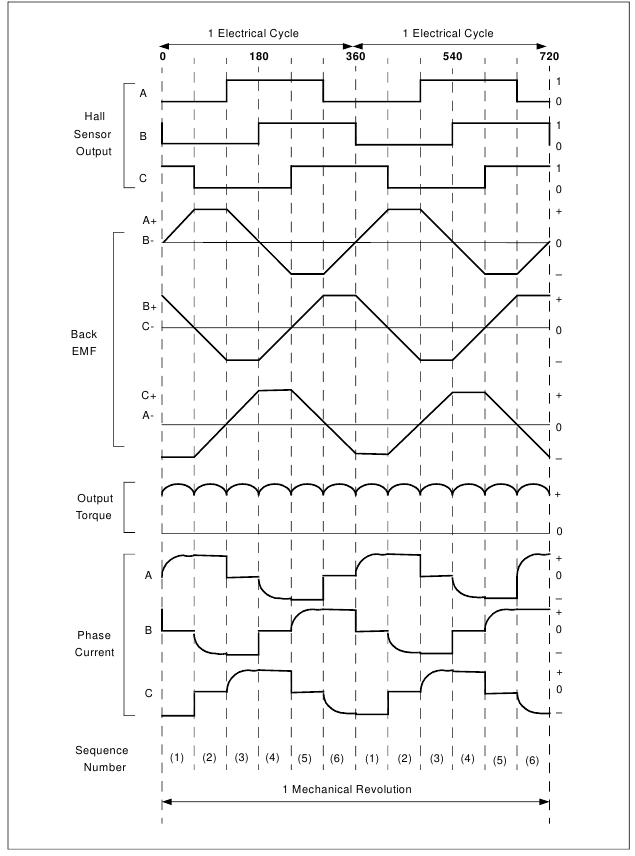
\includegraphics[width=5.5in]{images/signal.jpg}
	\caption{Hall effect sensors signal, back emf, output torque and phase current \citep{an885}}
	\label{im:signals}
\end{figure}

In this project, a PMBLDC hub motor is used as the sole powertrain of a electric vehicle. The electric vehicle will be used for participating in the Shell Eco-Marathon. It is a competition where teams compete for building the greatest mileage vehicle. The competition requires the participating teams to build their own car for the categories they are participating( for example, the urban concept category or the prototype category). For our case, a four-wheel electric vehicle is built for participation in urban concept category. The vehicle will be driven around a race track, which is the Sepang International Track, North Track for year 2012 for four laps with 10 seconds of stop between each lap. The total energy consumption of the vehicle after driving for 4 laps will be collected and the mileage will be calculated. Every team will have 3 attempts for mileage improvement.

\section{Problem Statement}
PMBLDC motor is better compare to brushed DC motor because brushless motor increases the efficiency by dropping the friction between the brush and the comutator which happens in brushed DC motor. However, the inefficient PWM in controlling the speed of the motor and the torque ripple cause by the phase current limits the efficiency of a PMBLDC motor.

There are three types of torque produced by a permanent magnet electric motor which are:

\begin{itemize}
	\item cogging torque
	\item reluctance torque
	\item mutual torque
\end{itemize}

The cogging torque is produced by the interaction between the permanent magnet at the rotor and the stator slots. Cogging torque is an undesireable torque generated by the electric motor which dominates at low speed and results in speed ripple. Cogging torque can only be minimize by means of hardware tuning which includes altering the number of poles, teeth at the stator or editing the controller setting which changes the drive current waveform.

The reluctance torque is generated by the difference in position of the rotor and the phase induction at the rotor. The ripple produced by the reluctance torque could be negligible with a good number of poles and slots of the windings at the stator.

The third type of torque produced by PMBLDC motor is the mutual torque which is caused by the non-sinusoidal signal reaching the stator windings or the magnet at the rotor. Since the torque is generated by the current, ripple reduction for mutual torque could be achieved by fine-tuning the current signal.

The torque ripple occurs in PMBLDC is mainly contributed by the different rise and decay time of the phase current as shown in figure \ref{im:signals}. The cogging torque does contribute to torque ripple in low speed but it's negligible at high speed. Torque ripple contributed by reluctance torque could also be ignored since the increasing number of poles and stator slot minimize the ripple. Mutual torque would be the major contributor to torque ripple due to the direct dependency on the current.

Based on figure \ref{im:comutation} (a), the rate of decay of $i_a$ is faster than the rate of increase of $i_b$. Therefore, at certain point where $i_a$ reaches 0 but $i_b$ still rising, there will be a surge in current at phase C, $i_c$. As the result, there will be a sudden drop in torque output. The same case happens as shown in figure \ref{im:comutation} (c) where $i_a$ drops slower than $i_b$ causing an sudden drop in $i_c$ and sudden increase in torque output. The same circumstances apply for $i_a$-$i_c$ and $i_b$-$i_c$ hence creating a ripple torque output. 

\begin{figure}[htb]
	\centering
	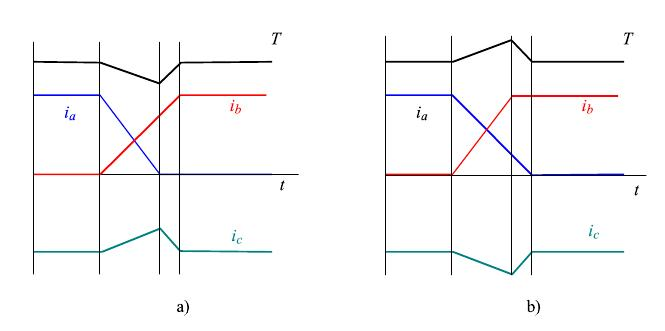
\includegraphics[width=5.5in]{images/phase_current.jpg}
	\caption{The phase current and torque during an alternating comutation event  \citep{7648}}
	\label{im:comutation}
\end{figure}

Apart from torque ripple in PMBLDC that reduce the efficiency of the electric motor and cut down the mileage of the electric vehicle, poor driving strategy will contribute to poor mileage. The Sepang North Track is a racing track that contains 3 uphill section and 3 uphill section and an approximately 800m long straight for the starting and ending line. This track is especially challenging for electric vehicle because the factor of torque generated by the electric motor, cruise speed when uphill and downhill, rolling resistance and drag factor need to be taken into consideration for minimum energy consumption.

\section{Objectives}

The objectives for this project are:

\begin{enumerate}
	\item To identify the output signal of the controller circuit and the hall effect sensor of the PMBLDC and develop a set of instrument for measuring the mileage of the electric vehicle.
	\item To study the track profile of Sepang North Track and create a simulation program for simulating the vehicle dynamics at the Sepang North Track.
	\item To compose a set of strategy to increase the mileage of the electric vehicle running on the Sepang North Track based using the simulation program.
\end{enumerate}

\section{Scope of Research}

In this project, the proprietary controller and PMBLDC motor signal output port will be identified. After that, by utilizing the signal output of the hall effect sensor and the controller speed output signal port, a set of instrument will be build for measuring the speed, input current and input voltage. The power input will then be calculated based on the voltage and current input.

Next up, the behaviour of the electric vehicle on the Sepang North Track will be simulated with taking the drag force, rolling resistance and track gradient into consideration. With the frontal area, coefficient of drag, coefficient of rolling resistance and the mass of the vehicle as manipulating variables, a set of strategies could be created for electric vehicle at different mass, tyre pressure at the same track with using the same electric motor as drive train.

\section{Research Approach}

For tapping the signal from the PMBLDC motor's hall effect sensors as well as the analog/digital output from the controller circuit board for the speed signal, multimeter will be used. For building the measurement tools for measuring and logging the input voltage, input current and the speed of the vehicle, Arduino boards will be used in conjunction with the self-made transducing circuit.

For simulating the vehicle's behaviour on track, self-made codes using C++ language will be used for iteration. Data for each set of simulation and strategies will be saved and the graph will be plot for analysing the effectiveness of the strategy.

\section{Summary}
In this chapter, the background of PMBLDC motor and the electric vehicle for participating in Shell Eco-Marathon has been introduced. Furthermore, the trapezoidal shape winding voltage for PMBLDC has been described and the use of hall effect sensor for detecting the position of the rotor is explained. 

The types of torque produced by PMBLDC motor is listed and the mutual torque has been identified as one of the problem contributor to the torque ripple for PMBLDC motor. The other problem raised up in this chapter is the poor racing strategy which cost us some mileage reduction during the Shell Eco-Marathon race.

The objectives for this project is listed which includes identifying the signal output of the proprietary controller and PMBLDC and build a measurement system for measuring the vehicle performance. Composing a set of strategies is one of the objectives listed.

Finally, the scope of the research has been limited to the study of the vehicle dynamics, electric motor and the Sepang North Track for building the simulation software which is a self-built software using C++ coding language. The measurement system will be built using the Arduino microcontroller which has the ability to measure, log and display the voltage, current and the velocity. 

\chapter{Literature Review}\label{chap:literature}

\chapter{Methodology}\label{chap:methodology}
\section{Introduction}
In this chapter, the procedure for tapping the signal from the proprietary controller and PMBLDC motor and then building a performance measurement system based on the identified signal will be listed. Furthermore, the process of developing the mathematical model and the simulation of electric vehicle on Sepang North Track will be described so that the optimal mileage strategy could be identified.

%%The terminology of this project is to hack and get the signal from a proprietary contoller and a PMBLDC hub motor, then a performance measurement system is built upon the signal obtained and then simulation is used for building optimal mileage strategy.

\section{Signal Identification}
The drive train of the electric vehicle that will be used for participation in Shell Eco-Marathon consists of a single hub motor with no transmission. The hub motor is a PMBLDC motor, hence a controller is needed for controlling the speed as well as running the hub motor. The controller has two parts which is the controller circuit that is responsible for signal handling and a power unit which receives the signal from the signal handling unit and create the phase current for running the PMBLDC.

The signal unit of the controller takes input signal from the throttle, the key and also the hall effect sensors signal from the PMBLDC motor before it can do the calculation and output the signal to the power unit. Apart from that, the signal unit of the controller powers the speedometer and delivers the signal (for example:  speed, battery voltage, vehicle mileage covered and the state of charge (SOC) of the battery ) for displaying at the speedometer.

Since the speedometer acts solely as a display unit, it does not have signal outputs or data logging capability. Logging the data manually by reading and recording the speed, voltage and SOC when the vehicle is running is appropriate because the electric vehilce is a single seater vehicle and it's impossible for the driver to drive and record the data simultaneously. 

Therefore, the signals need to be tapped from the signal unit of the controller in order to build a system that is able to measure, display and log the data needed. Tapping all the signals is redundant because some reading is primary (for example the voltage) whereas some readings are derived from the primary signal (for instance, the SOC of the battery is based on the voltage). Hence, identification of the primary signals should be adequate.

There are a few signal that need to be tapped from the controller and the PMBLDC motor such as:

\begin{itemize}
	\item{Speed from the controller}
	\item{Voltage from the controller}
	\item{Hall effect sensors signal from the PMBLDC motor}
\end{itemize}

Before the signal can be tapped and identified, the nature of the signal should be known. The voltage signal is an analog signal which is delivered directly from the battery through the controller. On the other hand, the speed signal should be an analog signal as well since the controller takes the signal of hall effect sensors, calculate the interval between each state change and multiply with the number of poles and the wheel diameter and get the speed of the vehicle as shown in equation \ref{eq:wheelSpeedHall}, where \textit{V} is the wheel speed, \textit{D} is the wheel diameter, \textit{N} is the number of poles of the PMBLDC motor and \textit{t} is the interval between changing state of the hall effect sensor.

\begin{equation}
	\label{eq:wheelSpeedHall}
	\text{\myequations{Wheel speed for direct drive based on hall effect sensor signal, wheel diameter and PMBLDC number of poles}}
	V = \frac{\pi D}{2Nt}
\end{equation}

Figure \ref{im:hall_signal} shows the hall effect signals which is a square wave. The hall effect sensor is a sensor where the output voltage from the sensor will change from minimum to maximum or vise versa depending on the circuit configuration. Since the sensor circuit is set in a way that it ampliefies the signal and output high/low when the magnetic field of the rotor is detected as shown in figure \ref{im:hall_circuit}, the signal output of the hall effect sensors is a square wave.

\begin{figure} [htb]
	\centering
	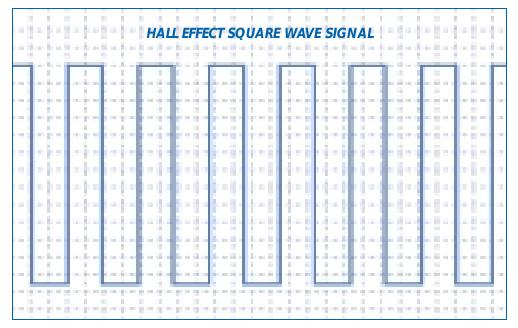
\includegraphics[width=3in]{images/hall_effect_signals.jpg}
	\caption{Hall effect sensor square wave signal \citep{counterpoint31}}
	\label{im:hall_signal}
\end{figure}

\begin{figure} [htb]
	\centering
	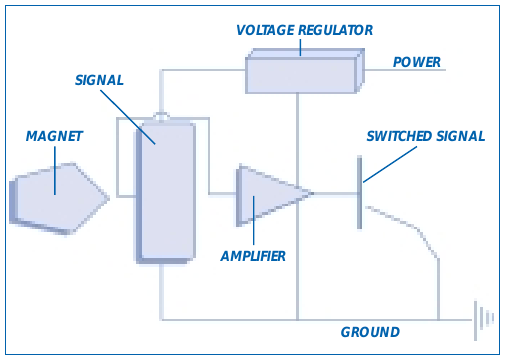
\includegraphics[width=3in]{images/hall_sensor_circuit.png}
	\caption{Circuit of hall effect sensor \citep{counterpoint31}}
	\label{im:hall_circuit}
\end{figure}

There are 16 ports for signal and power from the controller to the speedometer as shown in figure \ref{im:16pin}. The method for detecting the signal is trial and error and elimination. The ground port is found using the digital multimeter where the two probes of the digital multimeter is plug in to any 2 ports. The port where it is constantly lower voltage than the other 15 ports is the ground port.

\begin{figure} [htb]
	\centering
	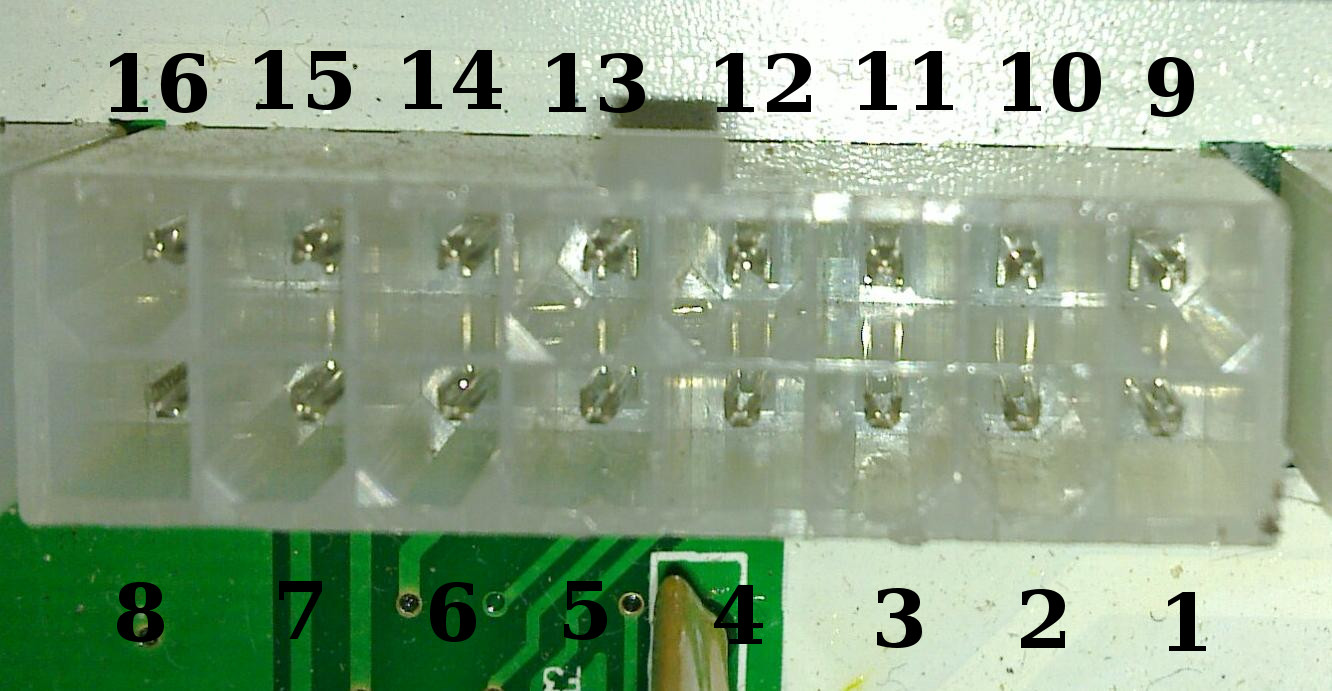
\includegraphics[width=4in]{images/16pin.jpg}
	\caption{16 pins controller circuit output}
	\label{im:16pin}
\end{figure}

After the ground port is found, the procedure above is repeated by testing the 15 ports by taking the ground port as reference. The voltage reading for those 15 ports is measured and recorded when the system is idle and when the motor is running. The ports for the following signal should be found:

\begin{itemize}
	\item{Speed where the reading changes when the motor is rotating and static}
	\item{Battery voltage which it is at ~50+V when the motor is idle and drops ~2V when the motor is running}
	\item{A constant voltage ~12V for powering the speedometer}
\end{itemize}

The hall effect sensor terminal is a 8 ports input/output as shown in figure \ref{im:hall8pin}. Again, the method for detecting the signal is trial and error with step by step elimination that is similar to the method used for identifying the speed signal at the controller circuit. The hall effect sensor circuit has the same circuit that is shown in figure \ref{im:hall_circuit} except that it has 3 sensors signal output instead of 1 output. 

\begin{figure} [htb]
	\centering
	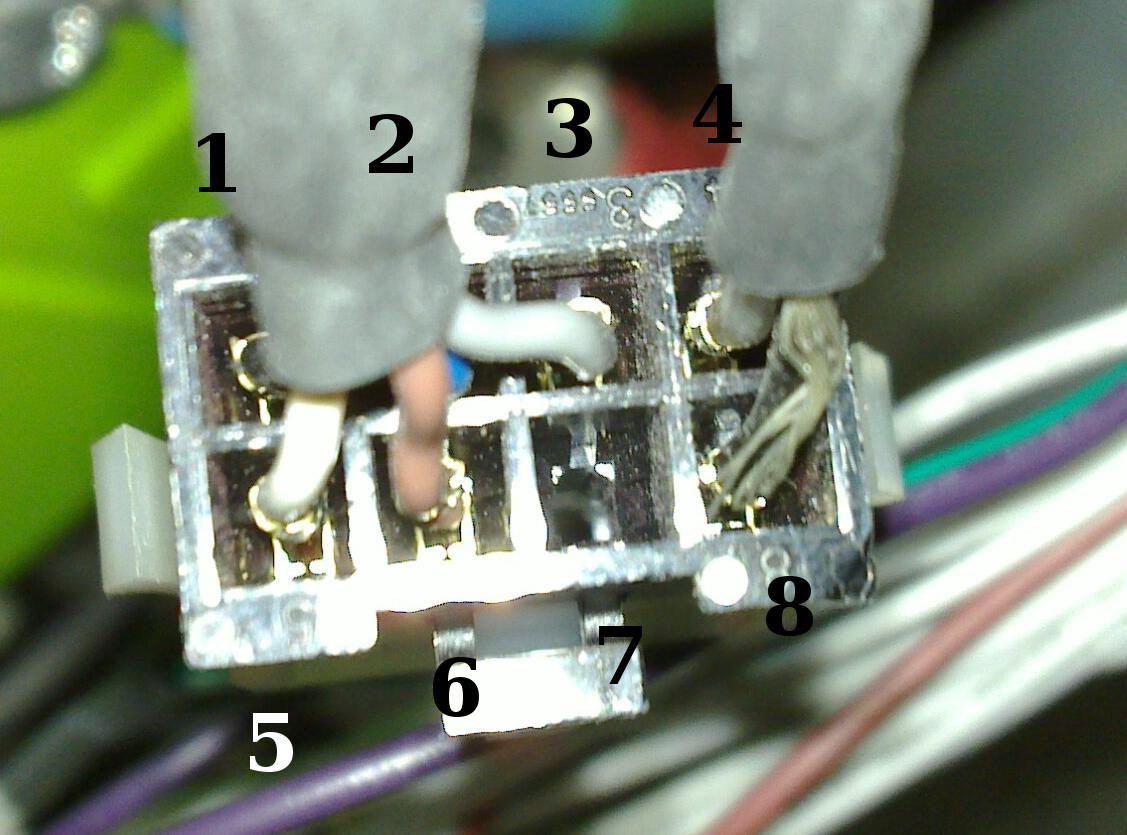
\includegraphics[width=4in]{images/hall.jpg}
	\caption{8 pins hall effect sensor I/O}
	\label{im:hall8pin}
\end{figure}

The hall effect sensor tapping is started with the identification of the voltage input to the hall effect sensors circuit. The voltage input to the circuit is 12V, hence, using the same method as speed signal detection, the digital multimeter's probe is plug into the any 2 ports of the 8 I/O ports within the terminal and detect the port with 12V reading.

After the voltage input ports is identified, the 3 hall effect sensors output signal is tapped by again plugging in the ground probe to the ground input port and the other positive probe to any 1 of the 6 remaining ports. The wheel is rotated manually over a revolution and the ports that produce ups and downs voltage signal would be the hall effect sensors output port.

After the hall effect sensors output port has been identified, the probes of the multimeter is plugged into the first hall effect sensor output port and the ground port. The wheel is rotated manually by hand over a revolution and the number of square wave over a wheel revolution is measured. 

\section{Measurement System}
After the primary signal (speed and voltage) is identified, a measurement that has the ability to measure, display and log the parameters need to be built. The purpose of building the measurement system is to

\begin{itemize}
	\item{Measure and log the power consumption of the electric vehicle so that the mileage of the vehicle can be known.}
	\item{Measure and log the power consumtion at each vehicle on-road speed.}
	\item{Building a speed and power consumption display for the electric vehicle.}
\end{itemize}

For measuring the power input, based on equation \ref{eq:powerInput}, the input voltage and input current need to be measured. Apart from measuring the power input to the electric vehicle, the data output from the measurement system can also be used to calculate the instantaneous deceleration of the vehicle when it's cruising, when it's braking with regenerative braking and when it's braking with regenerative and mechanical braking.

\begin{equation}
	\label{eq:powerInput}
	\text{\myequations{Power Input}}
	P_{input} = V_{input}I_{input}
\end{equation}

The measurement system uses a circuit with microcontroller, crystal and I/O pins, which is the Arduino Mega 2560 board for processing the signal from the controller circuit, calculate the real value based on the signal, log the data into a SD card through the ITDB02 shield and display the speed and power consumption value through the ITDB02-3.2(WC) LCD screen.

Since the microcontroller board can only accept I/O less than 5V and more than 0V but the battery voltage is in the range of 48V - 60V and the speed signal from the controller is negative voltage, hence an intermediate circuit has to be built so that the signal can be read by the microcontroller.

For the voltage measurement circuit, a voltage divider is built for measuring the voltage of the battery. The voltage divider is a 2 resistor circuit that has same or different value of resistance for each of the resistor as shown in figure \ref{im:voltageDivider} The voltage output, \textit{$V_{out}$} can be calculated using equation \ref{eq:voltageDivider} where \textit{R1} is the resistance for the first resistor, \textit{R2} is the resistance of the second resistor and \textit{$V_{in}$} is the voltage that need to be measured.

\begin{figure}[htb]
	\centering
	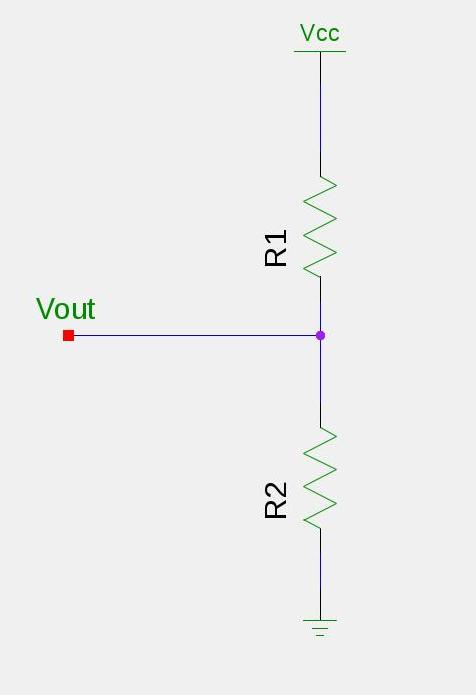
\includegraphics[width=3in]{images/voltage_divider.jpg}
	\caption{Voltage Divider}
	\label{im:voltageDivider}
\end{figure}

\begin{equation}
	\label{eq:voltageDivider}
	\text{\myequations{Voltage Divider}}
	V_{out} = \frac{V_{in}R2}{R1+R2}
\end{equation}

For measuring the speed, the same method which is the voltage divider is used with a little modification which replaces the \textit{$V_{in}$} to +5V and the ground to \textit{$V_{in}$} as shown in figure \ref{im:voltageDividerInverse} The \textit{$V_{out}$} for the modified voltage divider circuit could be calculated using equation \ref{eq:voltageDividerInverse}

\begin{figure}[htb]
	\centering
	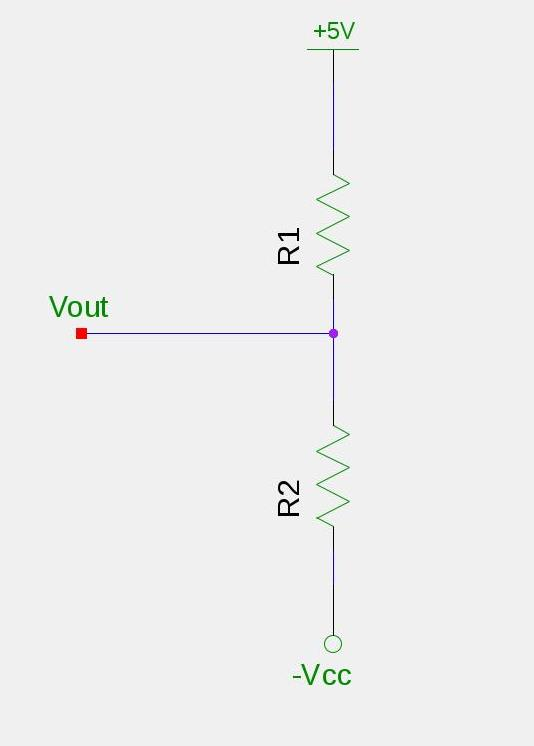
\includegraphics[width=3in]{images/voltage_divider_negative.jpg}
	\caption{Voltage Divider for negative voltage}
	\label{im:voltageDividerInverse}
\end{figure}

\begin{equation}
	\label{eq:voltageDividerInverse}
	\text{\myequations{Voltage Divider for negative voltage}}
	V_{out} = \frac{(5-V_{in})(R2)}{R1+R2} + V_{in}
\end{equation}

The resistance is selected based on the value of the negative voltage. For example, if the negative voltage is -5V, 1k\ohm \ resistor can be selected for both \textit{R1} and \textit{R2} which yields:

\centerline{$V_{out} = \frac{(5+5)(1000)}{1000+1000} - 5$}
\centerline{$V_{out} = 0V$}


If the \textit{$V_{in}$} is 0V, \textit{$V_{out}$} will be:

\centerline{$V_{out} = \frac{(5+0)(1000)}{1000+1000} - 0$}
\centerline{$V_{out} = 2.5V$}

Therefore, using a voltage divider, a negative voltage can be converted to positive voltage with minimum half of the original resolution.

The third parameter that need to be included in the measurement system is the input current. The input current is needed for calculating the input power to the electric vehicle and thus the overall vehicle mileage can be calculated. Since the rules of Shell Eco-Marathon restricted the nominal current input to the electric vehilce to be 60A and the peak current must be less than 150A, therefore a 200A current sensor is used.

The current sensor used in detecting the input current is the ALLEGRO MICROSYSTEMS ACS758ECB-200B-PFF-T which is a 200A current sensor with 5 terminals and analog voltage output signal. In order for the microcontroller to measure the current, a current measuring circuit with the current sensor is built.

After the prototype circuit of the current measuring circuit, the voltage measurement circuit and the speed voltage divider circuit is built, the 3 circuits is integrated into a single circuit and the microcontroller is program in a way that it can read, log and display the speed of the vehicle, the instantaneous current and voltage and the mileage covered every 100ms interval.

\section{Vehicle Simulation}
The purpose of simulating the vehicle behaviour on the Sepang North Track is to get a list of parameter so that the suitable battery could be selected as well as optimum power saving could be achieved. By simulating the vehicle running on the track, the instantaneous acceleration, speed, required torque, power output, current, total energy consumption and total time could be acquired.

Since there is no free software in the market currently that has the ability to simulate an electric vehicle and heavily customized for simulating the electric vehicle that would be used in Shell Eco-Marathon, a simulation software is written. 

The first step of building a simulation software is to build mathematical models for various components for vehicle dynamics. The mathematical model for the track and the PMBLDC motor need to be built so that the slope of the track and the power generation and consumption of the electric motor can be known.

\subsection{Track}
Figure \ref{im:trackGradient} shows the gradient of the track. By observing the graph, it can be seen that the maximum gradient is 5\% and the minimum gradient is -6\%. The gradient of the track can be discretized easily since the gradient is of integer value, meaning that it doesn't has 5.5\% gradient. From figure \ref{im:trackGradient} it also can be observed that the gradient has a minimum length of 25m and the length of each gradient is of n x 25m where n is any integer value, hence, a step of maximum 25m can be used to discretized the track gradient.

\begin{figure} [htb]
	\centering
	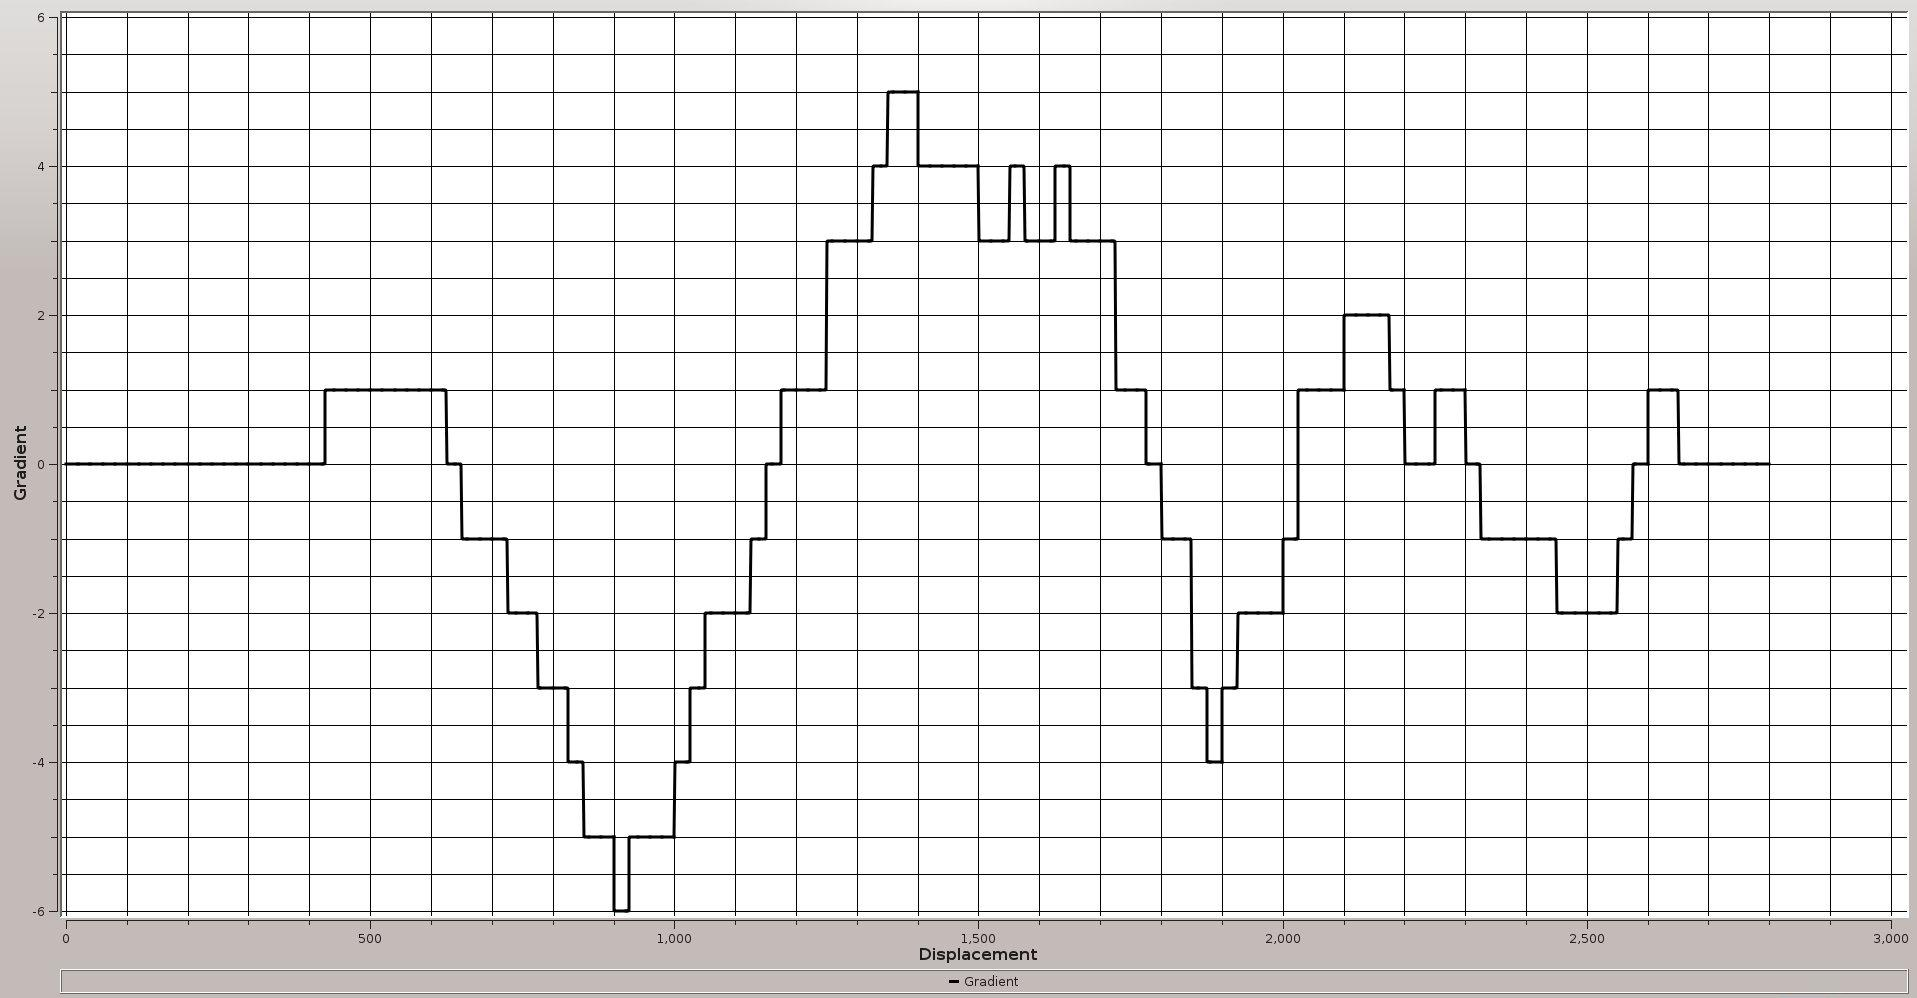
\includegraphics[width=6in]{images/track_gradient.jpg}
	\caption{Track gradient of Sepang North Track}
	\label{im:trackGradient}
\end{figure}

\subsection{Electric Motor}
Figure \ref{im:motorTorqueCurve} shows the torque and power output profile of the KLD D1064R electric motor. The reason the KLD D1064R is used in the simulation is because the proprietary PMBLDC used in the electric vehicle is manufactured by KLD and this motor is the most similar to the electric motor that is in used in terms of features, dimension and physical appearance. 

\begin{figure} [htb]
	\centering
	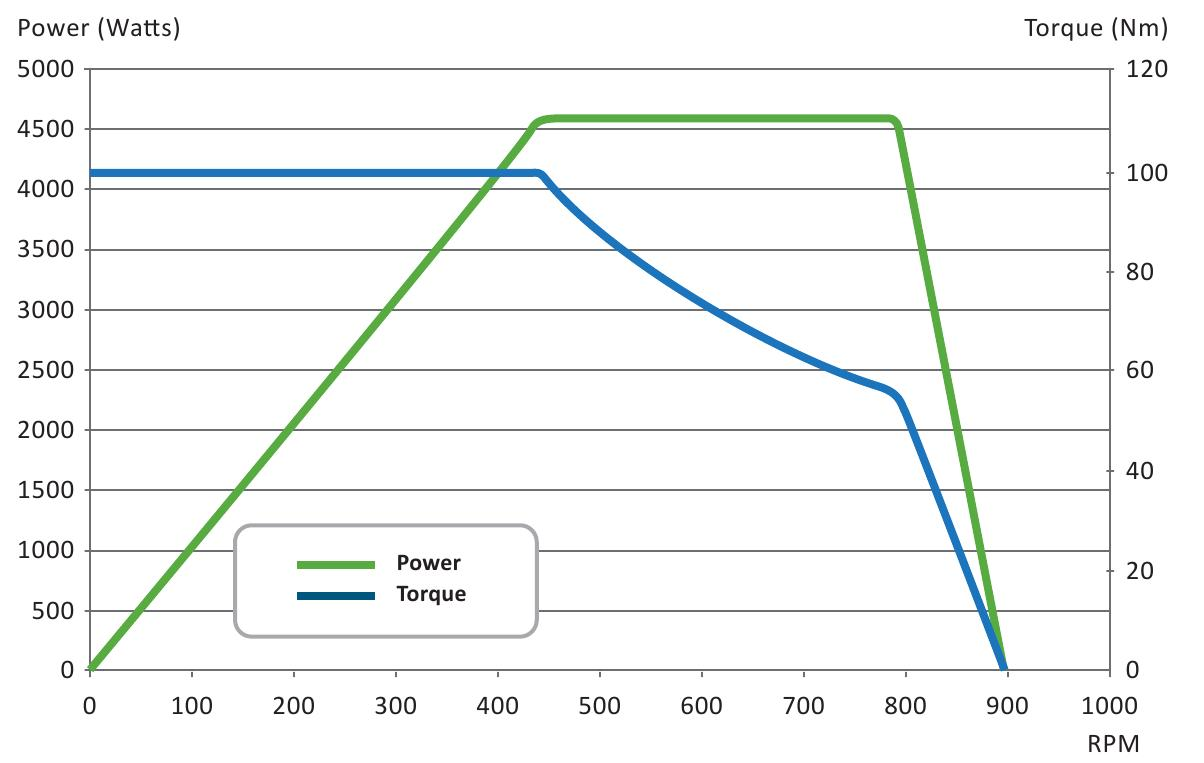
\includegraphics[width=6in]{images/kld_motor_torque_curve.jpg}
	\caption{Torque and power output curve for KLD D1064R \citep{kld}}
	\label{im:motorTorqueCurve}
\end{figure}

The torque curve can be discretized into the mathematical model shown in equation \ref{eq:motorTorqueModel}. Since the throttle is a torque type controller, therefore the torque generated by the electric motor can be calculated from the mathematical model for the torque of electric motor times the amount of throttle applied.

\begin{equation}
	\label{eq:motorTorqueModel}
	\text{\myequations{Mathematical model for the torque of the electric motor}}
	T = \begin{cases} 100 N.m, & \mbox{for (0 - 440 RPM)} \\ [0.0003(RPM)^2 - 0.493(RPM) + 260] N.m, & \mbox{for (441 - 800 RPM)} \\ [-0.56(RPM) + 504] N.m, & \mbox{for (801 - 900 RPM)} \end{cases}
\end{equation}

The power output curve of the electric motor shown in figure \ref{im:motorTorqueCurve} is the product of torque and rotational speed, which is represented in equation \ref{eq:powerOutputTorqueRPM} where \textit{$\tau$} is the torque and \textit{RPM} is the motor rotational speed at revolution per minute.

\begin{equation}
	\label{eq:powerOutputTorqueRPM}
	\text{\myequations{Relationship between power output, torque and rotational speed}}
	P_{output} = \frac{(\tau)(2\pi)(RPM)}{60000}
\end{equation}

\subsection{Air Drag Force}
The drag force by air drag exerted on a vehicle is directly proportional to the Coefficient of Drag (Cd), the frontal area of the vehicle, the density of the fluid, which in this context is the density of the air and also the square of the vehicle speed. By assuming the wind speed is 0 and no wind coming from any direction, the air drag force can be represented by the mathematical model shown in equation \ref{eq:airDragForce} where \textit{$\rho$} is the density of the air, \textit{$C_{d}$} is the coefficient of drag, \textit{A} is the frontal area of the vehicle and \textit{v} is the speed of the vehicle.

\begin{equation}
	\label{eq:airDragForce}
	\text{\myequations{Air drag force}}
	F_{drag} = \frac{1}{2}\rho C_{d} A v^2
\end{equation}

\subsection{Rolling Resistance}
The rolling resistance on the electric vehicle can be calculated using equation \ref{eq:rollingResistance} where \textit{mg} is the weight of the vehicle and \textit{$C_{rr}$} is the coefficient of rolling resistance of the vehicle.

\begin{equation}
	\label{eq:rollingResistance}
	\text{\myequations{Rolling resistance}}
	F_{roll} = mg C_{rr}
\end{equation}

\subsection{Slope}
When the vehicle is driving along a track that has lots of slope, for instance, the Sepang North Track, the uphill slopes will contribute to the resistance to the vehicle. The uphill and downhill force can be model using the equation \ref{eq:uphillForce} where \textit{mg} is the weight of the vehicle and \textit{$\theta$} is the angle of the slope in \textdegree .

\begin{equation}
	\label{eq:uphillForce}
	\text{\myequations{Uphill/downhill force}}
	F_{slope} = mgsin\theta
\end{equation}

\subsection{Vehicle Acceleration}
The acceleration of the vehicle can be calculated using the Newton's Second Law of motion which is shown in equation \ref{eq:newton2nd}. The parameter \textit{m} is the mass of the vehicle whereas the parameter \textit{a} is the acceleration of the vehicle.

\begin{equation}
	\label{eq:newton2nd}
	\text{\myequations{Newton's Second Law of Motion}}
	F = ma
\end{equation}

\subsection{Combine Mathematical Model}
After the mathematical model of the uphill/downhill, rolling resistance, air drag force and vehicle acceleration has been built, those mathematical equations are combined forming a combined mathematical model for simulation of vehicle dynamics. The combined mathematical model is shown in equation \ref{eq:combinedMath}. \textit{$\sum F_{resistance}$} is the total resistance force excerted to the electric vehicle. By ignoring the ambient temperature, weather condition and opposing wind speed, the mathematical model generated in equation \ref{eq:combinedMath} can be used to simulate the dynamics of the electric vehicle.

\begin{equation}
	\label{eq:combinedMath}
	\text{\myequations{Combined mathematical model for vehicle dynamics}}
	\sum F_{resistance} = mgsin\theta + mg C_{rr} + \frac{1}{2}\rho C_{d} A v^2 
\end{equation}

The acceleration or the decceleration of the electric vehicle can be calculated using equation \ref{eq:accelerationCalc}, where \textit{$\tau $} is the torque generated by the electric motor, \textit{R} is the radius of the wheel attached to the hub motor, \textit{$\sum F_{resistance}$} is the total resistance force calulated using equation \ref{eq:combinedMath} and \textit{m} is the total mass of the electric vehicle.

\begin{equation}
	\label{eq:accelerationCalc}
	\text{\myequations{Acceleration/Decceleration of the electric vehicle}}
	a = \frac{(\frac{\tau}{R} - \sum F_{resistance})}{m}
\end{equation}

\section{Summary}

The methodology for this project starts with the signal identification for the proprietary controller and PMBLDC motor. After the output signal for the speed and voltage has been identified, the voltage, current and speed measurement circuit has been built. The measurement circuit is able to measure, log the measurement result and display the parameters. Next, simulation program is built for simulating vehicle dynamics. With using the simulation program, a set of strategies can be composed.

\chapter{Result and Discussion}

\section{Introduction}

\section{Signal Identification}

\section{Measurement System}

\section{Vehicle Simulation}

\section{Strategies}

\section{Summary}

\chapter{Conclusion}

\section{Conclusion}
The signal for voltage, 12V supply voltage and the analog speed signal from the proprietary controller circuit has been identified. Apart from this, the hall effect sensors circuit pinout is identified and the number of poles of the electric motor is known by looking at the number of square wave per revolution of the hall effect sensor signal. The result for the number of poles for the PMBLDC motor is 28 poles.

Next, a measurement system that has the capability to measure the input voltage, input current and speed of the electric vehicle is made. The measurement system also features a SD card slot for logging the input voltage and current, and speed of the electric vehicle datas for future processing. Apart from that, the measurement circuit also act as a display console where the information of speed and system voltage can be delivered to the driver via an LCD display.

The simulation software is build based on the vehicle dynamics mathematical model which takes the rolling resistance, road slope, air drag and vehicle acceleration as parameters. The first strategy which is the "Full Throttle Everywhere" strategy is simulated and the resulting vehicle mileage is 18 km/Kwh. After that, "Preset Strategy 1" is created for tackling the energy wasted during downhill problem and the resulting mileage is improved to 27.62 km/kWh.

The strategy is further improved to "Preset Strategy 2" where the top speed is limited and vehicle cruising towards the end of the circuit which yields the mileage of 31.68 km/kWh. Finally, the "Preset Strategy 3" is introduces with gradual acceleration and dynamic required torque calculation and the result is further improved to 46.58 km/kWh.

To conclude, the objectives are achieved by successfully identified the signal output of the controller and PMBLDC motr and built a measurement system for measuring the required parameter. The simulation program is written and 4 strategies was composed with improvement between each strategy which matches the objective of this research paper.

\section{Future Works}
Since the controller and PMBLDC motor used in the electric vehicle is sponsored and hardware hacking is forbidden, it is recommended to tune the controller signal for reducing the torque ripple for future works. The controller output signal can be edited by modifying the hall effect sensors signal so that a lead/lag signal can be transmitted to the controller. By accepting the lead/lag hall effect sensors signal, the controller will produce shifted phase current. Hence by manipulating the hall effect sensors, the torque ripple caused by mutual torque in PMBLDC motor can be reduced.

Apart from tuning the drive electronically, the electric vehicle's mileage can be improved by improving the Coefficient of Drag of the electric vehicle. This is because from simulation result, the air-drag plays an important role in resisting the movement of the electric vehicle, hence, by reducing the $C_{d}$ and the frontal area, the mileage of the electric vehicle would be improved.

Lastly, the simulation software could be improved by including the environment variable (for example, the ambient temperature, rain and etc) and the vehicle mathematical model (for instance, the battery model, the PMBLDC motor model, the controller model, the tire pressure model and the battery temperature and discharge model). By improving the accuracy of the simulation software, accurate result can be simulated and better strategies could be tested and used for the future Shell Eco-Marathon racing.



\addtocontents{toc}{\protect\cftpagenumberson{chap}}

%%\ifpdf
%%  \pdfbookmark[-1]{Back Matter}{back}
%%\else\fi

\begin{singlespace}
%%%%%%%%%%%%%%%%%%%%%%%%%%%%%%%%%%%%%%%%%%%%%%%%%%%%%%%
% The bibliography.
% You can create mybib.bib with JabRef, the program included
% in the Colloquium05 CD-ROM.  Or download from
% http://jabref.sourceforge.net/
%%%%%%%%%%%%%%%%%%%%%%%%%%%%%%%%%%%%%%%%%%%%%%%%%%%%%%%
\bibliography{mybib}
\end{singlespace}

\addtocontents{toc}{\protect\setlength{\protect\cftbeforechapskip}{1pc}}


%%%%%%%%%%%%%%%%%%%%%%%%%%%%%%%%%%%%%%%%%%%%%%%%%%%%%%%
% The appendices.
% If you don't have any, you may delete everything below,
% until and including \chapter{Schematic}


.
%%%%%%%%%%%%%%%%%%%%%%%%%%%%%%%%%%%%%%%%%%%%%%%%%%%%%%%
%%\clearpage
%%\appendix
%%\phantomsection\addcontentsline{toc}{part}{\texorpdfstring{\uppercase{Appendices}}{Appendices}}
%%\thispagestyle{empty}
%%\vspace*{\stretch{1}}
%%  \begin{center}
%%    {\Huge\bfseries APPENDICES}
%%  \end{center}
%%\vspace*{\stretch{2}}
%%\addtocontents{toc}{\protect\renewcommand{\protect\chaptername}{\appendixname}} 
%%\addtocontents{toc}{\protect\setlength\cftchapnumwidth{7pc}}

%%\renewcommand\chaptername{\appendixname}
%%\chapter{Schematic}




%%%%%%%%%%%%%%%%%%%%%%%%%%%%%%%%%%%%%%%%%%%%%%%%%%%%%%%
% The list of own publications.  If you don't have one, you may
% comment out the next 3 lines (up till just before \end{singlespace}.
%%%%%%%%%%%%%%%%%%%%%%%%%%%%%%%%%%%%%%%%%%%%%%%%%%%%%%%
%%\nociteown{lim:2007,lim:latextypesetting}
%%\addtocontents{toc}{\protect\setlength{\protect\cftbeforechapskip}{3pc}}
%%\begin{singlespace}
%%\bibliographyown{mybib}
%%\end{singlespace}

\end{document}
